\begin{figure}[h!]
\centering
  \subfigure[$h_1$ ranges from 8 to 12.] {
    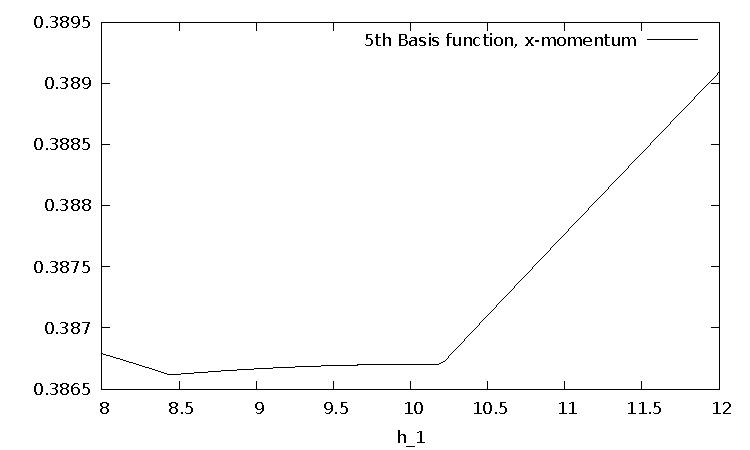
\includegraphics[scale=\zoomfactor]{{{ord2_magnitude_comparison_10_heights_momentums/y_12.0_7.0_15.0_11.0_9.0_-1.0_2.0_-3.0_4.0_-5.0_6.0_1.0_-2.0_3.0_-4.0_5.0_-6.0f08}}}
  }
  \subfigure[$h_1$ ranges from 8 to 12.] {
    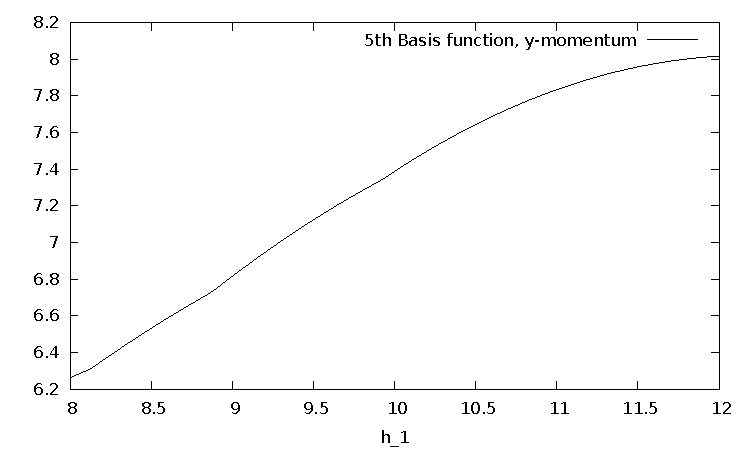
\includegraphics[scale=\zoomfactor]{{{ord2_magnitude_comparison_10_heights_momentums/y_12.0_7.0_15.0_11.0_9.0_-1.0_2.0_-3.0_4.0_-5.0_6.0_1.0_-2.0_3.0_-4.0_5.0_-6.0f09}}}
  }

  \subfigure[$h_1$ ranges from 998 to 1002.] {
    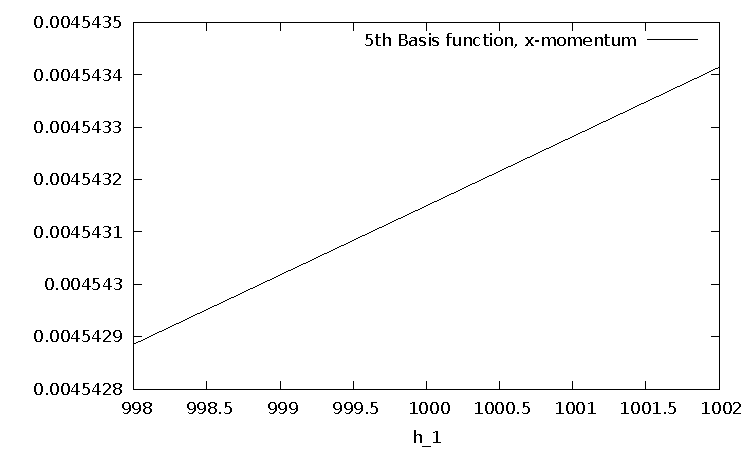
\includegraphics[scale=\zoomfactor]{{{ord2_magnitude_comparison_1000_heights_momentums/y_1002.0_997.0_1005.0_1001.0_999.0_-1.0_2.0_-3.0_4.0_-5.0_6.0_1.0_-2.0_3.0_-4.0_5.0_-6.0f08}}}
  }
  \subfigure[$h_1$ ranges from 998 to 1002.] {
    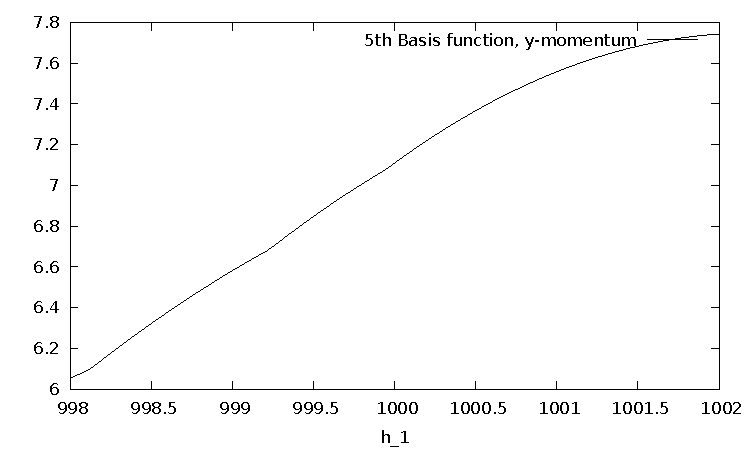
\includegraphics[scale=\zoomfactor]{{{ord2_magnitude_comparison_1000_heights_momentums/y_1002.0_997.0_1005.0_1001.0_999.0_-1.0_2.0_-3.0_4.0_-5.0_6.0_1.0_-2.0_3.0_-4.0_5.0_-6.0f09}}}
  }
\caption{Comparison of different orders of magnitude for differing heights and momentums. Heights are set to $h_2=12, h_3=7, h_4=15, h_5=11, h_6=9$, momentums to $u_{x,i}=(-1)^i \cdot i$ and $u_{y,i}=(-1)^{i+1} \cdot i$ for each plot.}
\label{fig:ord2_magnitude_comparison_heights_momentums}
\end{figure}

